\documentclass{article}
\usepackage[T1]{fontenc}
\usepackage{lmodern}
\usepackage{graphicx}
\usepackage{amsmath,amssymb}
\usepackage[a4paper,margin=2cm]{geometry}
\usepackage[absolute,overlay]{textpos}
\setlength{\TPHorizModule}{1mm}
\setlength{\TPVertModule}{1mm}
\usepackage[indonesian]{babel}
\usepackage{hyperref}
\setlength{\emergencystretch}{2em}
% unit: Halaman 7

\begin{document}

% === Halaman 7 (llm) ===

\vspace{163.35mm}

\begin{itemize}
    \item Top 10 huruf yang sering muncul dalam teks Bahasa Inggris: E, T, A, O, I, N, S, H, R, D, L, U
    \vspace{10mm}
    \item Top 10 huruf \textit{bigram} yang sering muncul dalam teks B. Inggris: TH, HE, IN, EN, NT, RE, ER, AN, TI, dan ES
    \item Top 10 huruf \textit{trigram} yang sering muncul dalam teks B. Inggris: THE, AND, THA, ENT, ING, ION, TIO, FOR, NDE, dan HAS
    \item Kriptanalis menggunakan tabel frekuensi kemunculan huruf dalam B. Inggris sebagai kakas bantu melakukan dekripsi.
    \item Misalnya, jika huruf ``R'' paling sering muncul di dalam cipherteks, maka kemungkinan besar itu adalah huruf ``E'' di dalam plainteksnya.
\end{itemize}

% deskripsi: Grafik batang yang menunjukkan frekuensi relatif kemunculan setiap huruf dalam alfabet Bahasa Inggris, dengan sumbu x berupa huruf (a-z) dan sumbu y berupa Relative Frequency (in percent).
% bbox normalisasi: [0.5400, 0.2200, 0.9600, 0.7700]
\begin{textblock*}{88.20mm}(113.40mm,65.34mm)
\noindent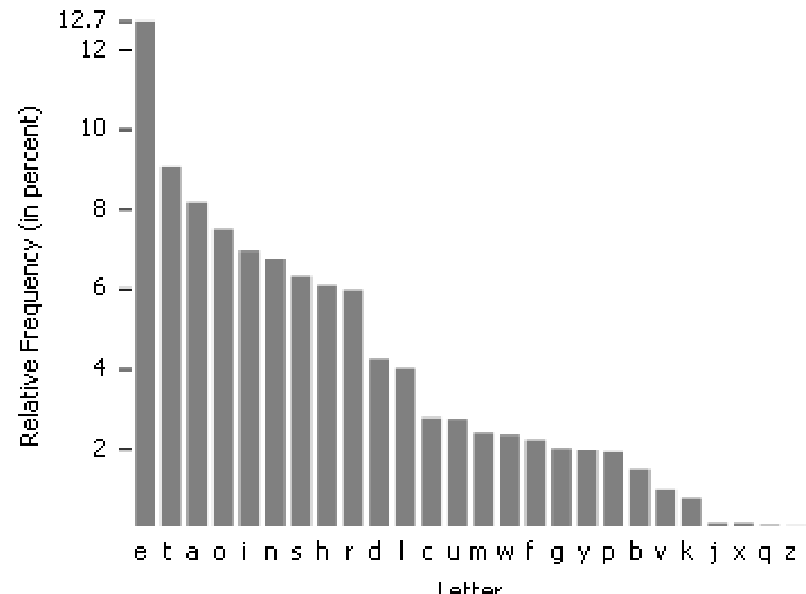
\includegraphics[width=88.20mm,height=163.35mm]{../../images/llm/page_007_img_01.png}%
\end{textblock*}

\end{document}
